\documentclass[tikz,border=10pt]{standalone}
\begin{document}
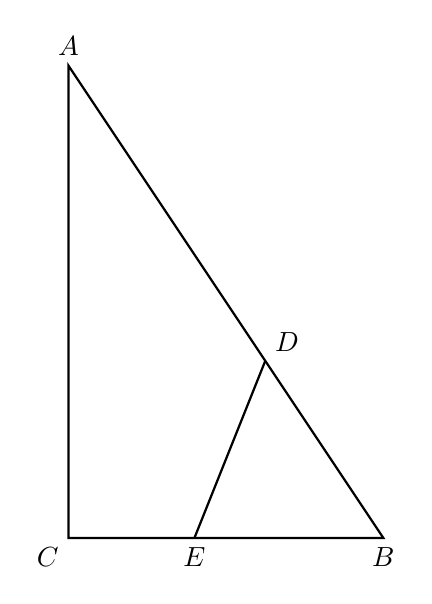
\begin{tikzpicture}
  \coordinate (C) at (0,0);
  \coordinate (A) at (0,6);
  \coordinate (B) at (4,0);
  \coordinate (D) at (2.5,2.25);
  \coordinate (E) at (1.6,0);

  \draw[thick] (A) -- (C) -- (B) -- cycle;
  \draw[thick] (E) -- (D);

  \node[above] at (A) {$A$};
  \node[above right] at (D) {$D$};
  \node[below] at (E) {$E$};
  \node[below left] at (C) {$C$};
  \node[below] at (B) {$B$};
\end{tikzpicture}
\end{document}
